\documentclass{standalone}
\usepackage{tikz}
\usetikzlibrary{patterns, positioning}

\begin{document}
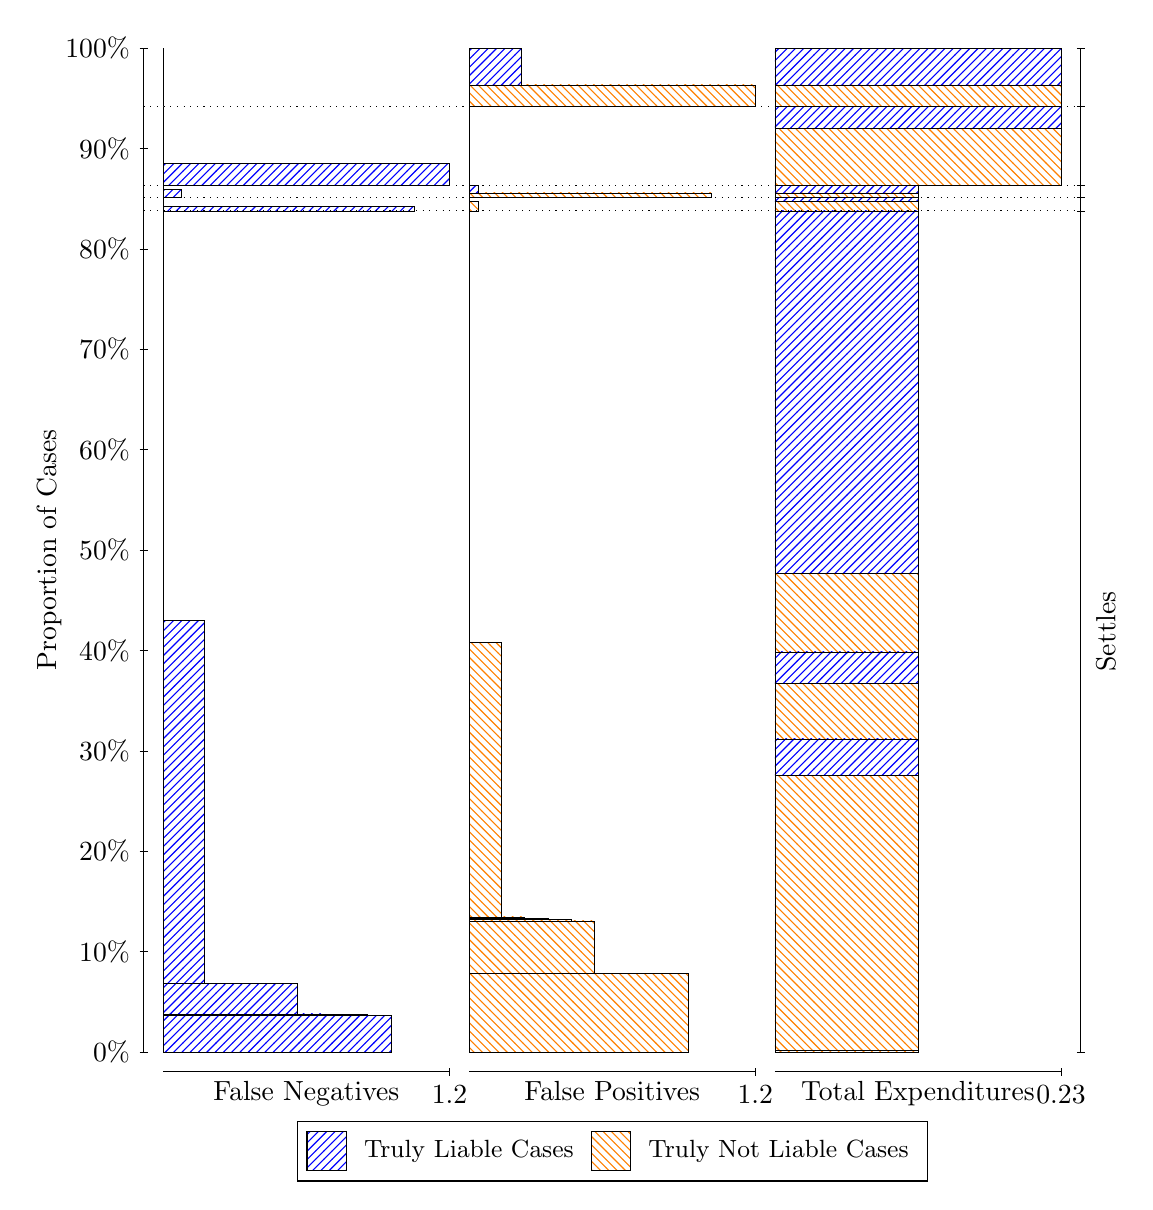
\begin{tikzpicture}
\draw[black, very thin] (1.5,1.75) -- (1.5,14.5);
\node[rotate=90, anchor=center] at (0.3, 8.125) {Proportion of Cases};
\draw[black, very thin] (1.45,1.75) -- (1.55,1.75);
\node[anchor=east] at (1.45, 1.75) {0\%};
\draw[black, very thin] (1.45,3.025) -- (1.55,3.025);
\node[anchor=east] at (1.45, 3.025) {10\%};
\draw[black, very thin] (1.45,4.3) -- (1.55,4.3);
\node[anchor=east] at (1.45, 4.3) {20\%};
\draw[black, very thin] (1.45,5.575) -- (1.55,5.575);
\node[anchor=east] at (1.45, 5.575) {30\%};
\draw[black, very thin] (1.45,6.85) -- (1.55,6.85);
\node[anchor=east] at (1.45, 6.85) {40\%};
\draw[black, very thin] (1.45,8.125) -- (1.55,8.125);
\node[anchor=east] at (1.45, 8.125) {50\%};
\draw[black, very thin] (1.45,9.4) -- (1.55,9.4);
\node[anchor=east] at (1.45, 9.4) {60\%};
\draw[black, very thin] (1.45,10.675) -- (1.55,10.675);
\node[anchor=east] at (1.45, 10.675) {70\%};
\draw[black, very thin] (1.45,11.95) -- (1.55,11.95);
\node[anchor=east] at (1.45, 11.95) {80\%};
\draw[black, very thin] (1.45,13.225) -- (1.55,13.225);
\node[anchor=east] at (1.45, 13.225) {90\%};
\draw[black, very thin] (1.45,14.5) -- (1.55,14.5);
\node[anchor=east] at (1.45, 14.5) {100\%};

\draw[black, very thin] (13.4,1.75) -- (13.4,14.5);
\draw[black, very thin] (13.35,1.75) -- (13.45,1.75);
\node[anchor=west] at (13.35, 1.75) {};
\draw[black, very thin] (13.35,12.433) -- (13.45,12.433);
\node[anchor=west] at (13.35, 12.433) {};
\draw[black, very thin] (13.35,12.607) -- (13.45,12.607);
\node[anchor=west] at (13.35, 12.607) {};
\draw[black, very thin] (13.35,12.759) -- (13.45,12.759);
\node[anchor=west] at (13.35, 12.759) {};
\draw[black, very thin] (13.35,13.758) -- (13.45,13.758);
\node[anchor=west] at (13.35, 13.758) {};
\draw[black, very thin] (13.35,14.5) -- (13.45,14.5);
\node[anchor=west] at (13.35, 14.5) {};

\draw[black, very thin, pattern color=blue, pattern=north east lines] (1.75,1.75) rectangle (4.6418,2.2171);
\draw[black, very thin, pattern color=blue, pattern=north east lines] (1.75,2.2171) rectangle (4.3452,2.2229);
\draw[black, very thin, pattern color=blue, pattern=north east lines] (1.75,2.2229) rectangle (4.0486,2.2288);
\draw[black, very thin, pattern color=blue, pattern=north east lines] (1.75,2.2288) rectangle (3.752,2.2348);
\draw[black, very thin, pattern color=blue, pattern=north east lines] (1.75,2.2348) rectangle (3.4554,2.6245);
\draw[black, very thin, pattern color=blue, pattern=north east lines] (1.75,2.6245) rectangle (2.269,7.2309);
\draw[black, very thin, pattern color=orange, pattern=north west lines] (1.75,7.2309) rectangle (1.75,12.433);
\draw[black, very thin, pattern color=blue, pattern=north east lines] (1.75,12.433) rectangle (4.9384,12.487);
\draw[black, very thin, pattern color=orange, pattern=north west lines] (1.75,12.487) rectangle (1.75,12.607);
\draw[black, very thin, pattern color=blue, pattern=north east lines] (1.75,12.607) rectangle (1.9724,12.705);
\draw[black, very thin, pattern color=orange, pattern=north west lines] (1.75,12.705) rectangle (1.75,12.759);
\draw[black, very thin, pattern color=blue, pattern=north east lines] (1.75,12.759) rectangle (5.3833,13.033);
\draw[black, very thin, pattern color=orange, pattern=north west lines] (1.75,13.033) rectangle (1.75,13.758);
\draw[black, very thin, pattern color=orange, pattern=north west lines] (1.75,13.758) rectangle (1.75,14.031);
\draw[black, very thin, pattern color=blue, pattern=north east lines] (1.75,14.031) rectangle (1.75,14.5);
\draw[black, very thin, pattern color=orange, pattern=north west lines] (5.6333,1.75) rectangle (8.4139,2.7465);
\draw[black, very thin, pattern color=orange, pattern=north west lines] (5.6333,2.7465) rectangle (7.2276,3.4148);
\draw[black, very thin, pattern color=orange, pattern=north west lines] (5.6333,3.4148) rectangle (6.931,3.4318);
\draw[black, very thin, pattern color=orange, pattern=north west lines] (5.6333,3.4318) rectangle (6.6344,3.4486);
\draw[black, very thin, pattern color=orange, pattern=north west lines] (5.6333,3.4486) rectangle (6.3378,3.4653);
\draw[black, very thin, pattern color=orange, pattern=north west lines] (5.6333,3.4653) rectangle (6.0412,6.9524);
\draw[black, very thin, pattern color=blue, pattern=north east lines] (5.6333,6.9524) rectangle (5.6333,12.433);
\draw[black, very thin, pattern color=orange, pattern=north west lines] (5.6333,12.433) rectangle (5.7446,12.554);
\draw[black, very thin, pattern color=blue, pattern=north east lines] (5.6333,12.554) rectangle (5.6333,12.607);
\draw[black, very thin, pattern color=orange, pattern=north west lines] (5.6333,12.607) rectangle (8.7105,12.661);
\draw[black, very thin, pattern color=blue, pattern=north east lines] (5.6333,12.661) rectangle (5.7446,12.759);
\draw[black, very thin, pattern color=orange, pattern=north west lines] (5.6333,12.759) rectangle (5.6333,13.484);
\draw[black, very thin, pattern color=blue, pattern=north east lines] (5.6333,13.484) rectangle (5.6333,13.758);
\draw[black, very thin, pattern color=orange, pattern=north west lines] (5.6333,13.758) rectangle (9.2667,14.031);
\draw[black, very thin, pattern color=blue, pattern=north east lines] (5.6333,14.031) rectangle (6.3007,14.5);
\draw[black, very thin, pattern color=orange, pattern=north west lines] (9.5167,1.75) rectangle (11.333,1.7667);
\draw[black, very thin, pattern color=blue, pattern=north east lines] (9.5167,1.7667) rectangle (11.333,1.7725);
\draw[black, very thin, pattern color=orange, pattern=north west lines] (9.5167,1.7725) rectangle (11.333,5.2596);
\draw[black, very thin, pattern color=blue, pattern=north east lines] (9.5167,5.2596) rectangle (11.333,5.7267);
\draw[black, very thin, pattern color=orange, pattern=north west lines] (9.5167,5.7267) rectangle (11.333,6.4288);
\draw[black, very thin, pattern color=blue, pattern=north east lines] (9.5167,6.4288) rectangle (11.333,6.8304);
\draw[black, very thin, pattern color=orange, pattern=north west lines] (9.5167,6.8304) rectangle (11.333,7.8269);
\draw[black, very thin, pattern color=blue, pattern=north east lines] (9.5167,7.8269) rectangle (11.333,12.433);
\draw[black, very thin, pattern color=orange, pattern=north west lines] (9.5167,12.433) rectangle (11.333,12.554);
\draw[black, very thin, pattern color=blue, pattern=north east lines] (9.5167,12.554) rectangle (11.333,12.607);
\draw[black, very thin, pattern color=orange, pattern=north west lines] (9.5167,12.607) rectangle (11.333,12.661);
\draw[black, very thin, pattern color=blue, pattern=north east lines] (9.5167,12.661) rectangle (11.333,12.759);
\draw[black, very thin, pattern color=orange, pattern=north west lines] (9.5167,12.759) rectangle (13.15,13.484);
\draw[black, very thin, pattern color=blue, pattern=north east lines] (9.5167,13.484) rectangle (13.15,13.758);
\draw[black, very thin, pattern color=orange, pattern=north west lines] (9.5167,13.758) rectangle (13.15,14.031);
\draw[black, very thin, pattern color=blue, pattern=north east lines] (9.5167,14.031) rectangle (13.15,14.5);
\draw[black, dotted] (1.5,12.433) -- (13.4,12.433);
\draw[black, dotted] (1.5,12.607) -- (13.4,12.607);
\draw[black, dotted] (1.5,12.759) -- (13.4,12.759);
\draw[black, dotted] (1.5,13.758) -- (13.4,13.758);
\draw[black, very thin] (1.75,1.5) -- (5.3833,1.5);
\node[anchor=north] at (3.5667, 1.5) {False Negatives};
\draw[black, very thin] (5.3833,1.45) -- (5.3833,1.55);
\node[anchor=north] at (5.3833, 1.45) {1.2};

\draw[black, very thin] (5.6333,1.5) -- (9.2667,1.5);
\node[anchor=north] at (7.45, 1.5) {False Positives};
\draw[black, very thin] (9.2667,1.45) -- (9.2667,1.55);
\node[anchor=north] at (9.2667, 1.45) {1.2};

\draw[black, very thin] (9.5167,1.5) -- (13.15,1.5);
\node[anchor=north] at (11.333, 1.5) {Total Expenditures};
\draw[black, very thin] (13.15,1.45) -- (13.15,1.55);
\node[anchor=north] at (13.15, 1.45) {0.23};

\node[black, centered, rotate=90] at (13.72, 7.0916) {Settles};





\draw (7.449999999999999,1.5) node[draw=none] (baseCoordinate) {};
\begin{scope}[align=center]
        \matrix[scale=0.5, draw=black, below=0.5cm of baseCoordinate, nodes={draw}, column sep=0.1cm]{
            \node[rectangle, draw, minimum width=0.5cm, minimum height=0.5cm, pattern=north east lines, pattern color=blue] {}; &
            \node[draw=none, font=\small] (B) {Truly Liable Cases}; &
            \node[rectangle, draw, minimum width=0.5cm, minimum height=0.5cm, pattern=north west lines, pattern color=orange] {}; &
            \node[draw=none, font=\small] (B) {Truly Not Liable Cases}; \\
            };
\end{scope}

\end{tikzpicture}
\end{document}